\documentclass[a4paper]{article}

%% Language and font encodings
\usepackage[english]{babel}
\usepackage[utf8x]{inputenc}
\usepackage[T1]{fontenc}

%% Sets page size and margins
\usepackage[a4paper,top=1.25cm,bottom=1.25cm,left=1.0cm,right=1.0cm,marginparwidth=1.25cm]{geometry}

%% Useful packages
\usepackage{amsmath}
\usepackage{graphicx}
\usepackage[colorinlistoftodos]{todonotes}
\usepackage[colorlinks=true, allcolors=blue]{hyperref}
\DeclareMathSizes{12}{30}{16}{12}
\usepackage[final]{pdfpages}
\usepackage{gensymb}
\usepackage{empheq}
\usepackage[section]{placeins}
\usepackage[most]{tcolorbox}
\usepackage{esint}
\usepackage{amssymb}
\usepackage{centernot}

\newcommand*\widefbox[1]{\fbox{#1}}
\newcommand{\eqComment}[1]{\text{  \# #1}}
\newcommand{\eqSep}{\text{ ;  }}
\newcommand{\experimental}{\text{!E||  }}
\newcommand{\sgn}[1]{sgn(#1)}
\newcommand{\n}{\\[1.5ex] \hline \nonumber \\[0ex]}
\newcommand{\m}{\nonumber \\}
\newcommand{\bij}{\stackrel{\sim}{\longrightarrow}}
\newcommand{\surj}{\twoheadrightarrow}
\newcommand{\inj}{\rightarrowtail}
\newcommand{\field}[1]{\textbf{\textit{#1}}}

\title{"The JP - Physics"}
\author{JP "The JP" Guzman}

\begin{document}
\maketitle
\allowdisplaybreaks

\section{Mathematics}
\subsection{Derivative definition and identities}
\begin{tcolorbox}[breakable, enhanced]
\begin{align}
   \frac{df(x)}{dx} = \frac{df}{dx} = \lim_{\Delta x \to 0} \frac{f(x + \Delta x) - f(x)}{\Delta x}
\n \frac{d(c(f(x))}{dx} = \lim_{\Delta x \to 0} \frac{c f(x + \Delta x) - c f(x)}{\Delta x} = c \lim_{\Delta x \to 0} \frac{f(x + \Delta x) - f(x)}{\Delta x} = c \frac{df}{dx}
\n \frac{d(f+g)}{dx} = \lim_{\Delta x \to 0} \frac{(f(x + \Delta x) + g(x + \Delta x)) - (f(x) + g(x))}{\Delta x} =
\m \lim_{\Delta x \to 0} \frac{f(x + \Delta x) - f(x)}{\Delta x} + \lim_{\Delta x \to 0} \frac{g(x + \Delta x) - g(x)}{\Delta x} = \frac{df}{dx} + \frac{dg}{dx}
\n \frac{df(g(x))}{dx} = \left(\frac{dg(x)}{dx}\right) \left(\frac{{df(g(x))}}{dg(x)}\right)
\end{align}
\end{tcolorbox}

\subsection{Differential equation identities}
For linear differential equations:
\begin{tcolorbox}[breakable, enhanced]
\begin{align}
   A(x) \frac{d^2y}{dx^2} + B(x) \frac{dy}{dx} + C(x) y = 0
\n A(x) \frac{d^2y_1}{dx^2} + B(x) \frac{dy_1}{dx} + C(x) y_1 = A(x) \frac{d^2y_2}{dx^2} + B(x) \frac{dy_2}{dx} + C(x) y_2 = 0
\n c_1 (A(x) \frac{d^2y_1}{dx^2} + B(x) \frac{dy_1}{dx} + C(x) y_1) + c_2 (A(x) \frac{d^2y_2}{dx^2} + B(x) \frac{dy_2}{dx} + C(x) y_2) = 0
\n A(x) (\frac{d^2(c_1 y_1)}{dx^2} + \frac{d^2(c_2 y_2)}{dx^2})) + B(x) (\frac{d(c_1 y_1)}{dx} + \frac{d(c_2 y_2)}{dx})) + C(x) (c_1 y_1 + c_2 y_2) = 0
\n (A(x) (\frac{d^2(c_1 y_1+ c_2 y_2)}{dx^2} + B(x) (\frac{d(c_1 y_1 + c_2 y_2)}{dx} + C(x) (c_1 y_1 + c_2 y_2) = 0) \implies (y = c_1 y_1 + c_2 y_2)
\end{align}
\end{tcolorbox}

\subsection{Integral and fundamental theorem of Calculus}
\begin{tcolorbox}[breakable, enhanced]
\begin{align}
   \int_{0}^{x_2} F(x) dx = G(x_2)
\n \int_{0}^{x_2 + \Delta x} F(x) dx = G(x_2 + \Delta x)
\n G(x_2 + \Delta x) - G(x_2) = F(x_2) \Delta x
\n F(x_2) = \frac{G(x_2 + \Delta x) - G(x_2)}{\Delta x}
\n F(x) = \frac{dG}{dx}
\n \sum_{i=1}^{n}(\Delta x_i) = \sum_{i=1}^{n}(x_i - x_{i-1}) = x_1 - x_0 + x_2 - x_1 + x_3 - x_2 + \ldots = -x_0 + x_n = x_n - x_0
\end{align}
\end{tcolorbox}

\subsection{Multivariable calculus}
\begin{tcolorbox}[breakable, enhanced]
\begin{align}
   \frac{\partial f(x, y)}{\partial x} = \frac{f_y(x)}{dx}
\n f(x + \Delta x, y + \Delta y) - f(x, y) = \left. \frac{\partial f}{\partial x} \right|_{x, y} \Delta x + \left. \frac{\partial f}{\partial y} \right|_{x + \Delta x, y} \Delta y
\n \Delta f = \left. \frac{\partial f}{\partial x} \right|_{x, y} \Delta x + (\left. \frac{\partial f}{\partial y} \right|_{x, y} + \left. \frac{\partial^2 f}{\partial x \partial y} \right|_{x, y} \Delta x) \Delta y
\n \Delta f = \left. \frac{\partial f}{\partial x} \right|_{x, y} \Delta x + \left. \frac{\partial f}{\partial y} \right|_{x, y} \Delta y + \left. \frac{\partial^2 f}{\partial x \partial y} \right|_{x, y} \Delta x \Delta y
\end{align}
\end{tcolorbox}

\subsection{Pythagoras theorem}
\begin{tcolorbox}[breakable, enhanced]
\begin{align}
   (a + b)^2 = 4 \left(\frac{a b}{2}\right) + c^2 = a^2 + b^2 + 2 a b = c^2 + 2 a b
\n c = \sqrt{a^2 + b^2}
\end{align}
\end{tcolorbox}

\subsection{Radians, angular and tangential velocity}
\begin{tcolorbox}[breakable, enhanced]
\begin{align}
   \Delta C = 2 \pi r \frac{\Delta \theta \degree}{360 \degree} = \left(\pi \frac{\Delta \theta \degree}{180 \degree}\right) r = \Delta \theta r
\n V_r = \frac{d\theta}{dt} = \omega
\n V_C = \frac{dC}{dt} = r \omega
\end{align}
\end{tcolorbox}

\subsection{Vector products, sum and product identities}
\begin{tcolorbox}[breakable, enhanced]
\begin{align}
   |r| = \sqrt{r_x(\theta)^2 + r_y(\theta)^2}
\n \cos(\theta) = \frac{r_x(\theta)}{|r|} \eqSep \sin(\theta) = \frac{r_y(\theta)}{|r|} \eqSep \tan(\theta) = \frac{r_y(\theta)}{r_x(\theta)}
\n \hyperlink{pdfs/idns-proof.pdf}{\textbf{Proof for sum and difference identities: idns-proof.pdf}}
\n \hyperlink{pdfs/FormulaSheet.pdf}{\textbf{Sum and product identities: FormulaSheet.pdf}}
\n \vec{A} \cdot \vec{B} = A_x B_x + A_y B_y = |A| \cos(\theta_A) |B| \cos(\theta_B) + |A| \sin(\theta_A) |B| \sin(\theta_B) = 
\m |A| |B| (\cos(\theta_A) \cos(\theta_B) + \sin(\theta_A) \sin(\theta_B)) = |A| |B| \cos(\theta) \eqComment{dot product or magnitude product}
\n \vec{A} \times \vec{B} = |A| |B| \sin(\theta) \hat{\perp}(\theta) \eqComment{cross product or vector product}
\n \vec{A} \times \vec{B} = \vec{A} \cdot \vec{B} \tan(\theta) \hat{\perp}(\theta)
\end{align}
\end{tcolorbox}

\subsection{Taylor series and exponential function expansion}
\begin{tcolorbox}[breakable, enhanced]
\begin{align}
   f(x) \approx f(0) \approx f(0) + x \frac{df}{dx}(0) \approx f(0) + x \frac{df}{dx}(0) + \left(\frac{x^2}{2!}\right) \frac{d^2f}{dx^2}(0) \eqComment{factorials annihilate discrepancies}
\n f(x) = \sum_{n=0}^{\infty} \left(\frac{x^n}{n!}\right) \left(\frac{d^nf}{dx^n}(0)\right) \eqComment{derivatives at $x=0$ extrapolates $f(x)$ as it deviates from $x=0$}
\n e^x = 1 + x + \frac{x^2}{2!} + \frac{x^3}{3!} + \frac{x^4}{4!} + \frac{x^5}{5!} + \frac{x^6}{6!} + \ldots
\n \sin(x) = x - \frac{x^3}{3!} + \frac{x^5}{5!} - \frac{x^7}{7!} + \ldots
\n \cos(x) = 1 - \frac{x^2}{2!} + \frac{x^4}{4!} - \frac{x^6}{6!} + \ldots
\n e^{ix} = 1 + i x + \frac{i^2 x^2}{2!} + \frac{i^3 x^3}{3!} + \frac{i^4 x^4}{4!} + \frac{i^5 x^5}{5!} + \frac{i^6 x^6}{6!} + \ldots = \cos(x) + i \sin(x)
\n e^{ix} + e^{-ix} = (\cos(x) + i \sin(x)) - (\cos(x) - i \sin(x)) = 2 \cos{x}
\n \cos(x) = \frac{e^{ix} + e^{-ix}}{2} \eqSep \sin(x) = \frac{e^{ix} + e^{-ix}}{2 i}
\end{align}
\end{tcolorbox}

\subsection{Complex numbers}
\begin{tcolorbox}[breakable, enhanced]
\begin{align}
   z = x + i y \eqSep z^\star = x - i y
\n z_1 + z_2 = x_1 + i y_1 + x_2 + i y_2 = (x_1 + x_2) + i (y_1 + y_2)
\n (z_1) (z_2) =  (x_1 + i y_1) (x_2 + i y_2) = x_1 x_2 + i x_1 y_2 + i y_1 x_2 + i^2 y_1 y_2 = (x_1 x_2 - y_1 y_2) + i (x_1 y_2 + y_1 x_2)
\n Re(z) = \frac{z + z^\star}{2} = x
\n Im(z) = \frac{z - z^\star}{2 i} = y
\n z z^\star = (x^2 - (-y^2)) + i (x (-y) + y x) = x^2 + y^2 = {|z|}^2 \eqComment{magnitude squared of z}
\n \frac{z_1}{z_2} = \left(\frac{x_2 + i y_2}{x_1 + i y_1}\right) \left(\frac{x_1 - i y_1}{x_1 - i y_1}\right) = \frac{(x_2 + i y_2) (x_1 - i y_1)}{{x_1}^2 + {y_1}^2}
\n x = r \cos(\theta) \eqSep y = r \sin(\theta)
\n z = x + i y = r (\cos(\theta) + i \sin(\theta)) = |z| e^{i \theta}
\end{align}
\end{tcolorbox}

\section{Classical Mechanics}
\subsection{Force, work, kinetic energy, Work-Energy theorem}
\begin{tcolorbox}[breakable, enhanced]
\begin{align}
   \experimental F = m \frac{d^2x}{dt^2} = \frac{dp}{dt} = m \frac{dv}{dt} = m a
\n SI(F) = (kg) m / s^2 = N = \textbf{Netwons}
\n \Delta W = F \Delta x \eqComment{force inducing a displacement}
\n SI(W) = (kg) m^2 / s^2 = N m = J = \textbf{Joules}
\n P = \frac{\Delta W}{\Delta t} = F \frac{\Delta x}{\Delta t} = F v
\n SI(P) = (kg) m^2 / (s^2 t) = W / t = \textbf{Watt}
\n m \frac{dv}{dt} v = m \frac{d \frac{v^2}{2}}{dt} = m a v = m a \frac{dx}{dt}
\n  \frac{m}{2} {v_2}^2 - \frac{m}{2} {v_1}^2 = m a (x_2 - x_1)
\n K = \frac{1}{2} m v^2 \eqComment{energy associated with motion}
\n SI(K) = SI(W)
\n K_2 - K_1 = F (x_2 - x_1) = W_2 - W_1
\n \Delta K = F \Delta x = \Delta W
\n v^2 = {v_x}^2 + {v_y}^2
\n \frac{dK}{dt} = \frac{d\left(\frac{m v^2}{2}\right)}{dt} = \frac{m d({v_x}^2 + {v_y}^2)}{2 dt} = \frac{m (2 v_x \frac{dv_x}{dt}+ 2 v_y \frac{dv_y}{dt})}{2} = m \frac{dv_x}{dt} v_x + \frac{dv_y}{dt} m v_y = F_x v_X + F_y v_y = \vec{F} \cdot \vec{v}
\n dW = dt \frac{dK}{dt} = dt (F_x v_x + F_y v_y) = dt (F_x \frac{dr_x}{dt} + F_y \frac{dr_y}{dt}) = F_x dr_x + F_y dr_y = \vec{F} \cdot d\vec{r}
\end{align}
\end{tcolorbox}

\subsection{Potential energy, energy conservation}
\begin{tcolorbox}[breakable, enhanced]
\begin{align}
   K_2 - K_1 = \int_{x_1}^{x^2} F(x) dx = G_2 - G_1 = U_1 - U_2
\n U = - \int F dx \eqComment{energy associated with position}
\n K_2 + U_2 = K_1 + U_1 = E \eqComment{energy conservation}
\n SI(U) = SI(F x) = SI(K) = SI(E)
\n \frac{\partial^2 U}{\partial y \partial x} = \frac{\partial F_x}{\partial y} = \frac{\partial F_y}{\partial x} = \frac{\partial^2 U}{\partial x \partial y} \eqComment{multivariable conservative force?}
\end{align}
\end{tcolorbox}

\subsection{Gravity and inclined plane}
\begin{tcolorbox}[breakable, enhanced]
\begin{align}
   \vec{F_g} = -\frac{g M_1 M_2}{{r_{1,2}}^2} \left(\frac{\vec{r}}{|r|}\right) = -\frac{g M m}{{r}^2} \hat{r}
\n (m a_x \hat{x} + m a_y \hat{y}) = (m g \sin(\theta) \hat{x} + (N - m g \cos(\theta))\hat{y})
\end{align}
\end{tcolorbox}

\begin{figure}[h]
\centering
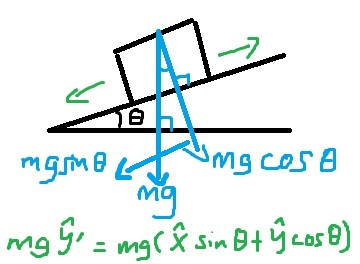
\includegraphics[width=0.35\textwidth]{figures/mgtheta.jpg}
\caption{\label{fig:mgtheta}This mgtheta was uploaded via the project menu.}
\end{figure} \FloatBarrier

\subsection{Circular motion}
\begin{tcolorbox}[breakable, enhanced]
\begin{align}
   T = \frac{2 \pi}{\left(\frac{\Delta \theta}{\Delta t}\right)} = \frac{2 \pi}{\omega}
\n V_C = \frac{2 \pi r}{T} = \omega r
\n \vec{x}(t) = |r| (\hat{x} \cos(\omega t) + \hat{y} \sin(\omega t))
\n \vec{v}(t) = \omega |r| (-\hat{x} \sin(\omega t) + \hat{y} \cos(\omega t))
\n \vec{a}(t) = -\omega^2 |r| (+\hat{x} \cos(\omega t) + \hat{y} \sin(\omega t))
\end{align}
\end{tcolorbox}

\subsection{Multiple body system}
\begin{tcolorbox}[breakable, enhanced]
\begin{align}
   \vec{F_{a, b}} = -\vec{F_{b, a}} 
\n \frac{\vec{F_{a, b}}}{\Delta t} = \frac{-\vec{F_{b, a}}}{\Delta t} = \vec{p_{a, b}} = -\vec{p_{b, a}}
\n \frac{d\vec{p_{a, b}}}{dt} = \frac{d(-\vec{p_{b, a}})}{dt}
\n \frac{d\vec{p_{a, b}}}{dt} + \frac{d(-\vec{p_{b, a}})}{dt} = \frac{d(\vec{p_{a, b}} + \vec{p_{b, a}})}{dt} = 0 \eqComment{momentum conservation}
\n M = m_1 + m_2
\n X = \frac{m_1 x_1 + m_2 x_2}{M} \eqComment{Center of mass}
\n m_1 \frac{d^2 \vec{x_1}}{dt^2} + m_2 \frac{d^2 \vec{x_2}}{dt^2} = F_{1,2} + F_{1,e} + F_{2,1} + F_{2,e} = F_{1,e} + F_{2,e} = 
\m F_e = M \frac{d^2 \vec{X}}{dt^2} \eqComment{Center of mass motion depends solely on external forces}
\n X = \frac{\int_0^L M x \frac{dx}{L}}{M} = \frac{1}{L} \int_0^L x dx = \frac{L}{2}
\end{align}
\end{tcolorbox}

\begin{figure}[h]
\centering
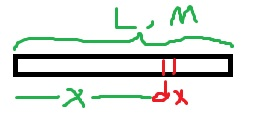
\includegraphics[width=0.3\textwidth]{figures/continuousrod.jpg}
\caption{\label{fig:continuousrod}This continuousrod was uploaded via the project menu.}
\end{figure} \FloatBarrier

\subsection{Rigid body system}
\begin{tcolorbox}[breakable, enhanced]
\begin{align}
   I = \sum_i^n m_i {r_i}^2 \eqComment{moment of intertia or rotational inertia}
\n SI(I) = (kg) m^2
\n L = I \omega \eqComment{angular momentum}
\n SI(L) = SI(I \omega) = (kg) m^2 / t
\n \alpha = \frac{d\omega}{dt} = \frac{d^2\theta}{dt^2} \eqComment{angular acceleration}
\n SI(\alpha) = SI(L / t) = (kg) m^2 / t^2
\n \omega^2 = {\omega_0}^2 + 2 \alpha(\theta - \theta_0)
\n K = \frac{1}{2} \sum_i^n m_i {v_i}^2 = \frac{1}{2} \sum_i^n m_i {r_i}^2 \omega^2 = \frac{1}{2} I \omega^2 
\n \Delta W = F \Delta x = F (r \Delta \theta)
\n \Delta K = \frac{1}{2} I(\omega^2 - {\omega_0}^2) = \frac{1}{2} I({\omega_0}^2 + 2 \alpha(\theta_0 - \theta) - {\omega_0}^2) = I \alpha \Delta \theta
\n \frac{\Delta W}{\Delta \theta} = \frac{\Delta K}{\Delta \theta} = F r = I \alpha = \frac{dL}{dt} = \tau \eqComment{torque}
\n SI(\tau) = SI(F x)
\n \vec{L} = \vec{r} \times \vec{p} \eqComment{multivariable axis and speed of rotation}
\n \vec{\tau} = \frac{d\vec{L}}{dt} = \frac{d\vec{r}}{dt} \times \vec{p} + \vec{r} \times \frac{d\vec{p}}{dt} = \vec{v} \times \vec{p} + \vec{r} \times \vec{F} = \vec{v} \times m \vec{v} + \vec{r} \times \vec{F} = \vec{r} \times \vec{F}
\end{align}
\end{tcolorbox}

\subsection{Multiple rigid body system}
\begin{tcolorbox}[breakable, enhanced]
\begin{align}
   \tau = F r = \sum_i (F_i - N_i) r_i = \sum_i (F_i (\cos(\theta_i) + \sin(\theta_i)) - F_i \cos(\theta_i)) r_i = \sum_i F_i \sin(\theta_i) r_i
\n \sum_i \frac{m_i \vec{r_{{CM}_i}}}{M} = 0 \eqComment{origin is at the center of mass}
\n \sum_i \frac{m_i \vec{r_{{CM}_i}}}{M \Delta t} = \sum_i \frac{m_i \vec{v_{{CM}_i}}}{M} = \sum_i \vec{p_{{CM}_i}} = 0
\n I_{CM} = \sum_i m_i \vec{r_{{CM}_i}}^2
\n I = \sum_i m_i \vec{r_i}^2 = \sum_i m_i (\vec{d} + \vec{r_{{CM}_i}})^2 = \sum_i m_i \vec{d}^2 + 2 \vec{d} \sum_i m_i \vec{r_{{CM}_i}} + \sum_i m_i \vec{r_{{CM}_i}}^2 =
\m M d^2 + 2 \vec{d} \sum_i m_i \vec{r_{{CM}_i}} + I_{CM} = M d^2 + 2 M \vec{d} \sum_i \frac{m_i \vec{r_{{CM}_i}}}{M} + I_{CM} = M d^2 + I_{CM}
\n K = \frac{1}{2} \sum_i^n m_i v_i = \frac{1}{2} \sum_i^n m_i (v_{CM} + v_{i-CM})^2 = 
\m \frac{1}{2} \sum_i^n (m_i {v_{CM}}^2 + m_i {v_{i-CM}}^2 + 2 m_i v_{CM} v_{i-CM}) = 
\m \frac{1}{2} M v_{CM} + \frac{1}{2} I_{CM} \omega^2 + v_{CM} \sum_i^n m_i v_{{CM}_i} = \frac{1}{2} M v_{CM} + \frac{1}{2} I_{CM} \omega^2 = K_{{CM}_T} + K_{{CM}_R}
\end{align}
\end{tcolorbox}

\subsection{Stationary ladder}
\begin{tcolorbox}[breakable, enhanced]
\begin{align}
   w - f = 0 \eqSep N - M g = 0 \eqComment{equilibrium constraints}
\n w L \sin(\theta) = M g \frac{L}{2} \sin(\frac{\pi}{2} - \theta) = M g \frac{L}{2} \cos(\theta)
\n w = \frac{M g}{2} \cot(\theta) = f \leq \mu_S N \leq \mu_S M g
\n \cot(\theta) \leq 2 \mu_S \implies \tan(\theta) \geq \frac{1}{2 \mu_S}
\end{align}
\end{tcolorbox}

\begin{figure}[h]
\centering
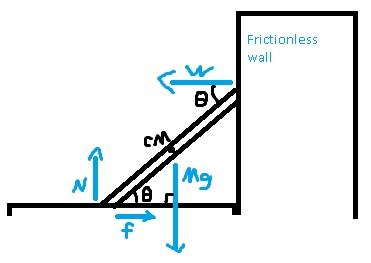
\includegraphics[width=0.6\textwidth]{figures/ftauequilibrium.jpg}
\caption{\label{fig:ftauequilibrium}This ftauequilibrium was uploaded via the project menu.}
\end{figure} \FloatBarrier

\section{Relativity}
\subsection{Lorentz transformations}
\begin{tcolorbox}[breakable, enhanced]
\begin{align}
   S = (x, t) \eqSep S^\prime = (x^\prime, t^\prime) \eqSep x = x^\prime = t = t^\prime = 0 \eqComment{light pulse event from origin}
\n \experimental x^\prime = (x - u t) \gamma \eqSep x = (x^\prime + u t^\prime) \gamma \eqComment{inertial coordinate transform postulate}
\n \experimental x = c t \eqSep x^\prime = c t^\prime \eqComment{EM relativity postulate}
\n c = \frac{t}{x} = \frac{t^\prime}{x^\prime}
\n x^\prime x = (x x^\prime + x u t^\prime - x^\prime u t - u^2 t t^\prime) \gamma^2
\n \gamma^2 = \frac{1}{(1 + u \frac{t^\prime}{x^\prime} - u \frac{t}{x} - \frac{u^2 t t^\prime}{x x^\prime})} = \frac{1}{1 - u^2 \frac{t}{x} \frac{t^\prime}{x^\prime}} = \frac{1}{1 - \frac{u^2}{c^2}} \implies \gamma = \frac{1}{\sqrt{1 - \frac{u^2}{c^2}}}
\n t^\prime = \frac{1}{u} \left(\frac{x}{\gamma} - x^\prime\right) = \frac{1}{u} \left(\frac{x}{\gamma} - \gamma(x - u t)\right) = \frac{\gamma}{u} \left(\frac{x}{\gamma^2} - x + u t\right) = \frac{\gamma}{u} (x(1 - \frac{u^2}{c^2}) - x + u t) =
\n \frac{\gamma}{u} (u t - x\frac{u^2}{c^2}) = \gamma (t - x\frac{u}{c^2}) = \frac{t - x\frac{u}{c^2}}{\sqrt{1 - \frac{u^2}{c^2}}} \eqComment{x', t' are linear combinations of x, t}
\n \Delta x^\prime = {x^\prime}_2 - {x^\prime}_1 = (\Delta x - u \Delta t) \gamma
\n \Delta t^\prime = (\Delta t - u \frac{\Delta x}{c^2}) \gamma
\n v^\prime = \frac{\Delta x^\prime}{\Delta t^\prime} = \frac{\Delta x - u \Delta t}{\Delta t - u \frac{\Delta x}{c^2}} = \frac{v - u}{1 - u \frac{v}{c^2}} 
\end{align}
\end{tcolorbox}

\subsection{Dependent events}
\begin{tcolorbox}[breakable, enhanced]
\begin{align}
   (\sgn{\Delta t^\prime} = - \sgn{\Delta t}) \implies (u \frac{\Delta x}{c^2} > \Delta t) \implies (1 > \frac{u}{c} > \frac{c \Delta t}{\Delta x}) \implies (\Delta x > c \Delta t)
\n (\sgn{\Delta t^\prime} = \sgn{\Delta t}) \implies (\Delta x < c \Delta t) \eqComment{dependent events are in range of light signal propagation}
\end{align}
\end{tcolorbox}

\subsection{Distance in space-time}
\begin{tcolorbox}[breakable, enhanced]
\begin{align}
   \beta = \frac{u}{c}
\n {x_0}^\prime = c t^\prime = \frac{c t - c \frac{x}{c} \frac{u}{c}}{\sqrt{1 - \beta^2}} = \frac{x_0 - \beta x_1}{\sqrt{1 - \beta^2}} \eqComment{time-like component}
\n {x_1}^\prime = x^\prime = \frac{x_1 - \beta x_0}{\sqrt{1 - \beta^2}} \eqComment{space-like component}
\n {{x_0}^\prime}^2 - {{x_1}^\prime}^2 = \frac{{x_0}^2 + \beta^2 {x_1}^2 - 2 x_0 \beta x_1 - {x_1}^2 - \beta^2 {x_0}^2 + 2 x_1 \beta x_0}{1 - \beta^2} =
\n \frac{{x_0}^2 (1 - \beta^2) - {x_1}^2 (1 - \beta^2)}{1 - \beta^2} = {x_0}^2 - {x_1}^2 = S^2 \eqComment{space-time interval}
\n X = (x_0, \vec{r}) = (x_0, x_1 ,x_2, x_3) = (c t, \vec{r}) \eqComment{space-time four-vector}
\n L_a \cdot L_b = l_{a_0} l_{b_0} - l_{a_1} l_{b_1} - l_{a_2} l_{b_2} - l_{a_3} l_{b_3} \eqComment{four-vector dot product}
\n X^2 = X \cdot X = {x_0}^2 - {|\vec{r}|}^2 = {x_0}^2 - {x_1}^2 - {x_2}^2 - {x_3}^2 = S^2
\end{align}
\end{tcolorbox}

\begin{figure}[h]
\centering
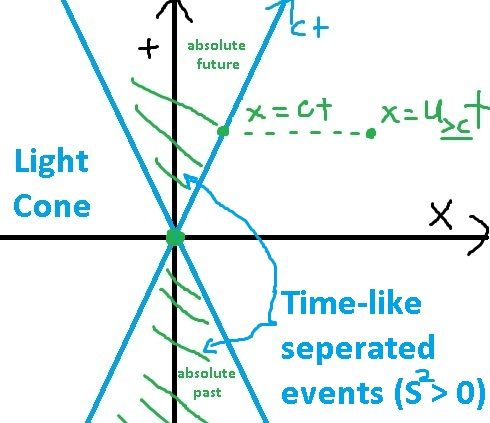
\includegraphics[width=0.40\textwidth]{figures/lightcone.jpg}
\caption{\label{fig:lightcone}This lightcone was uploaded via the project menu.}
\end{figure} \FloatBarrier

\subsection{Vectors in space-time}
\begin{tcolorbox}[breakable, enhanced]
\begin{align}
   (\Delta S^\prime)^2 = (\Delta S)^2 = (c \Delta t)^2 - (\Delta x)^2 = (c \Delta t)^2 - (\Delta x)^2 = (c \Delta t)^2 (1 - \frac{v^2}{c^2})
\n \Delta S = \sqrt{(c \Delta t)^2 - (\Delta x)^2} = c \Delta t \sqrt{1 - \frac{{\Delta x}^2}{{\Delta t}^2 c^2}} = c \Delta t \sqrt{1 - \frac{v^2}{c^2}}
\n \tau \implies \Delta x = 0 \eqSep v = 0 \eqComment{scalar proper time in the reference frame of the object}
\n \Delta S = c \Delta t \sqrt{1 - \frac{v^2}{c^2}} = c \Delta \tau \sqrt{1 - \frac{0}{c^2}} = c \Delta \tau
\n \frac{dt}{d\tau} = \frac{1}{\sqrt{1 - \frac{v^2}{c^2}}} = \gamma
\n V = \frac{dX}{d\tau} = \frac{dX}{dt} \frac{dt}{d\tau} = \frac{dX}{dt} \gamma = \left(\frac{d(ct)}{dt}, \frac{d\vec{r}}{dt}\right) \gamma = \frac{1}{\sqrt{1 - \frac{v^2}{c^2}}} \left(c, \frac{d\vec{r}}{dt}\right) \eqComment{vector via scaling with an invariant}
\n P = m_0 V = m_0 \frac{1}{\sqrt{1 - \frac{v^2}{c^2}}} \left(c, \frac{d\vec{r}}{dt}\right) = \left(\frac{m_0 c}{\sqrt{1 - \frac{v^2}{c^2}}}, \frac{m_o \vec{v}}{\sqrt{1 - \frac{v^2}{c^2}}}\right) = (P_0, P_1, P_2, P_3)
\n c P_0 = \frac{c m_0 c}{\sqrt{1 - \frac{v^2}{c^2}}} =  c m_0 c (1 - \frac{v^2}{c^2})^{\frac{-1}{2}} =
\n c m_0 c \left(1 \left(\frac{1}{0!}\right) + \left(\frac{-1}{2}\right) \left(\frac{-v^2}{c^2}\right) \left(\frac{1}{1!}\right) + \left(\frac{-1}{2}\right) \left(\frac{-1}{2} - 1\right) \left(\frac{-v^2}{c^2}\right)^2 \left(\frac{1}{2!}\right) + \ldots \right) =
\n \left(m_0 c^2 +\frac{1}{2} m_0 v^2 + \frac{3}{8} m_0 \frac{v^4}{c^2} + \ldots \right) = E_0
\n P = \left(\frac{E_0}{c}, \frac{\vec{p}}{\sqrt{1 - \frac{v^2}{c^2}}}\right) \eqComment{energy-momentum four-vector}
\n P \cdot P = \left(\frac{m c}{1 - \frac{v^2}{c^2}}\right)^2 - \left(\frac{m v}{1 - \frac{v^2}{c^2}}\right)^2 = \frac{m^2 c^2 - m^2 v^2}{1 - \frac{v^2}{c^2}} = m^2 c^2
\n P \cdot P = {P_0}^2 - {P_1}^2 = \left(\frac{E}{c}\right)^2 - {P_1}^2 = m^2 c^2
\n E^2 = m^2 c^4 + p^2 c^2 \eqComment{energy-mass equivalence}
\n \frac{d P}{d \tau} = 0 \eqComment{invariant energy-momentum conservation}
\end{align}
\end{tcolorbox}

\subsection{Photon energy-momentum conservation}
\begin{tcolorbox}[breakable, enhanced]
\begin{align}
   \experimental K = \left(\frac{\omega}{c}, \vec{K}\right) \eqSep \omega = |\vec{K}| c \eqComment{photon energy-momentum four-vector}
\n K \cdot K = \left(\frac{\omega}{c}\right)^2 - \vec{K} \cdot \vec{K} = |\vec{K}|^2 - |\vec{K}|^2 = 0 = m_K^2 c^2 = 0 c^2 = 0
\n P_b = P_a + K
\n \left(\frac{m_b c}{\sqrt{1 - \frac{v^2}{c^2}}}, \frac{m_b v}{\sqrt{1 - \frac{v^2}{c^2}}}\right) = (m c, 0) + \left(\frac{\omega}{c}, \vec{K}\right)
\n \frac{m_b c}{\sqrt{1 - \frac{v^2}{c^2}}} = m c + \frac{\omega}{c} \eqSep \frac{m_b v}{\sqrt{1 - \frac{v^2}{c^2}}} = 0 + \vec{K}
\n{P_b}^2 = m_b^2 c^2 = (P_a + K)^2 = P_a^2 + K^2 + 2 P_a k = {m_a}^2 c^2 + 0 + 2 (m_a c, 0) \cdot \left(\frac{\omega}{c}, \vec{K}\right) =
\n {m_a}^2 c^2 + 2 m_a \omega = {m_b}^2 c^2 \eqComment{bypasses $v$ terms}
\n m_b = \sqrt{{m_a}^2 + \frac{2 m_a \omega}{c^2}}
\n v = \vec{K} \frac{\sqrt{1 - \frac{v^2}{c^2}}}{m_b} = \vec{K} \frac{\sqrt{1 - \frac{v^2}{c^2}}}{\sqrt{{m_a}^2 + \frac{2 m_a \omega}{c^2}}}
\end{align}
\end{tcolorbox}

\subsection{Particle collision producing additional particles}
\begin{tcolorbox}[breakable, enhanced]
\begin{align}
   P_E + P_{r} = \left(\frac{E}{c}, \vec{P}\right) + (m c, 0) = 4 (m c, \vec{P_f}) \eqComment{case: when 2 masses + energy = 4 masses}
\n \left(\left(\frac{E}{c}, \vec{P}\right) + (m c, 0)\right)^2 =  (4 (m c, 0))^2 = 16 m^2 c^2
\n \left(\frac{E}{c} + m c, \vec{P}\right)^2 = \left(\frac{E}{c} + m c\right)^2 - \vec{P}^2 = \frac{E^2}{c^2} + m^2 c^2 + 2 E m - p^2 =
\n 2 m^2 c^2 + p^2 + 2 E m - p^2 = m^2 c^2 + 2 E m = 16 m^2 c^2
\n E = 7 m c^2
\end{align}
\end{tcolorbox}

\section{Harmonic Motion}
\subsection{Mass and spring system}
\begin{tcolorbox}[breakable, enhanced]
\begin{align}
   m \frac{d^2 x}{dt^2} = -k x \eqComment{harmonic motion with spring constant $k$}
\n \omega_0 = \sqrt{\frac{k}{m}} \eqComment{natural frequency of a mass and spring system ?}
\n \frac{d^2 x}{dt^2} = -\frac{k}{m} x = -{\omega_0}^2 x
\n x = A e^{\alpha t} \eqComment{guess solution}
\n \alpha^2 A e^{\alpha t} + {\omega_0}^2 A e^{\alpha t} = 0
\n (A (\alpha^2 + {\omega_0}^2) e^{\alpha t} = 0) \implies \forall_t ( (A=0) \lor (\alpha^2 + {\omega_0}^2 = 0) ) \implies (\alpha = \pm i \omega_0)
\n x_1 = A_1 e^{+i \omega_0 t} \eqSep x_2 = A_2 e^{-i \omega_0 t}
\n x = A_1 e^{i \omega t} + A_2 e^{-i \omega t} \eqSep \omega = \sqrt{\frac{k}{m}}
\n x = x^\star = A_1 e^{i \omega t} + A_2 e^{-i \omega t} = {A_1}^\star e^{-i \omega t} + {A_2}^\star e^{i \omega t} \implies A_1 = {A_2}^\star \eqComment{assume $x$ is real}
\n x = A e^{i \omega_0 t} + A^\star e^{-i \omega_0 t} = |A| e^{i \phi} e^{i \omega_0 t} + |A| e^{-i \phi} e^{-i \omega_0 t} = |A| e^{i (\omega_0 t + \phi)} + |A| e^{-i (\omega_0 t + \phi)} =
\n 2 |A| \cos(\omega t + \phi) = C \cos(\omega t + \phi)
\end{align}
\end{tcolorbox}

\subsection{Mass and spring system with friction}
\begin{tcolorbox}[breakable, enhanced]
\begin{align}
\n m \frac{d^2x}{dt^2} = -k x - \mu \frac{dx}{dt} \eqComment{harmonic motion with friction $\mu$}
\n m \frac{d^2x}{dt^2} + k x + \mu \frac{dx}{dt} = 0
\n \frac{d^2x}{dt^2} + \frac{k}{m} x + \left(\frac{\mu}{m}\right) \frac{dx}{dt} = \frac{d^2x}{dt^2} + {\omega_0}^2 x + \gamma \frac{dx}{dt} = 0
\n (x = A e^{\alpha t}) \implies (A (\alpha^2 + \alpha \gamma + {\omega_0}^2) (e^{\alpha t}) = 0)
\n \alpha^2 + \alpha \gamma + {\omega_0} = 0
\n \alpha = \frac{-\gamma \pm \sqrt{\gamma^2 - 4 {\omega_0}^2}}{2} = -\frac{\gamma}{2} \pm \sqrt{\left(\frac{\gamma}{2}\right)^2 - {\omega_0}^2} = \alpha_\pm
\n x = A e^{\alpha_+ t} + B e^{\alpha_- t} = A e^{-\left(\frac{\gamma}{2} - \sqrt{\left(\frac{\gamma}{2}\right)^2 - {\omega_0}^2}\right) t} + B e^{-\left(\frac{\gamma}{2} + \sqrt{\left(\frac{\gamma}{2}\right)^2 - {\omega_0}^2}\right) t}
\n (\frac{\gamma}{2} > \omega_0) \implies (\sgn{\alpha_+} = \sgn{\alpha_-} = 1) \eqComment{over-damped relaxation}
\n v = \frac{dx}{dt} = \alpha_+ A e^{\alpha_+ t} + \alpha_- B e^{\alpha_- t}
\n x(0) = A + B \eqSep v(0) = \alpha_+ A + \alpha_- B
\n (\frac{\gamma}{2} < \omega_0) \implies (\alpha = -\frac{\gamma}{2} \pm \sqrt{\left(\frac{\gamma}{2}\right)^2 - {\omega_0}^2}) = -\frac{\gamma}{2} \pm i \sqrt{{\omega_0}^2 - \left(\frac{\gamma}{2}\right)^2}) \eqComment{damped oscillation}
\n \omega^\prime = (\sqrt{{\omega_0}^2 - \left(\frac{\gamma}{2}\right)^2} \eqComment{damped frequency of a mass and spring system with friction}
\n x = A e^{-\left(\frac{\gamma t}{2} - i \sqrt{{\omega_0}^2 - \left(\frac{\gamma}{2}\right)^2}\right)} + B e^{-\left(\frac{\gamma t}{2} + i \sqrt{{\omega_0}^2 - \left(\frac{\gamma}{2}\right)^2}\right)} = 
\n (A + B) e^{-\frac{\gamma}{2} t} \cos\left(\left(\sqrt{{\omega_0}^2 - \left(\frac{\gamma}{2}\right)^2}\right) t + \phi\right) = (A + B) e^{-\frac{\gamma}{2} t} \cos\left(\omega^\prime t + \phi\right)
\end{align}
\end{tcolorbox}

\subsection{Mass and spring system with friction and driving force}
\begin{tcolorbox}[breakable, enhanced]
\begin{align}
   m \left(\frac{d^2x}{dt^2} + \mu \frac{dx}{dt} + k x\right) = F \cos(\omega t) \eqComment{harmonic motion with a driving force $F$ and driving frequency $\omega$}
\n (F \cos(\omega t) = 0) \implies \left(\frac{d^2{x_c}}{dt^2} + \gamma \frac{d{x_c}}{dt} + {\omega_0}^2 {x_c} = 0\right) \implies ({x_c} = A e^{i \alpha t}) \eqComment{solution annihilated by operators}
\n \left(\frac{\gamma}{2} > \omega_0\right) \implies \left(\alpha = -\frac{\gamma}{2} \pm \sqrt{{\frac{\gamma}{2}}^2 - {\omega_0}^2}\right)
\n \left(\frac{\gamma}{2} < \omega_0\right) \implies \left(\alpha = -\frac{\gamma}{2} \pm i \sqrt{{\omega_0}^2 - {\frac{\gamma}{2}}^2} = -\frac{\gamma}{2} \pm i \omega^\prime\right)
\n {x_c} = A_1 e^{-\frac{\gamma t}{2}} e^{i \omega^\prime t} +  A_2 e^{-\frac{\gamma t}{2}} e^{-i \omega^\prime t} = |A| e^{i \phi_0} (e^{i} + e^{-i}) = 2 |A| e^{-\frac{\gamma t}{2}} \cos(\omega^\prime t + \phi_0)
\n (F \cos(\omega t) \neq 0) \implies \left(\frac{d^2x}{dt^2} + \gamma \frac{dx}{dt} + {\omega_0}^2 x = \frac{F}{m} \cos(\omega t)\right)
\n \left(\frac{d^2z}{dt^2} + \gamma \frac{dz}{dt} + {\omega_0}^2 z = \frac{F}{m} (\cos(\omega t) + i \sin(\omega t)) = \frac{F}{m} e^{i \omega t}\right) \implies (x = Re(z))
\n z = z_0 e^{i \omega t}
\n (-\omega^2 + \omega \gamma + {\omega_0}^2) z_0 e^{i \omega t} = \frac{F}{m} e^{i \omega t}
\n z_0 = \frac{\left(\frac{F}{m}\right)}{-\omega^2 + \omega \gamma + {\omega_0}^2}
\n z = \frac{\left(\frac{F}{m} e^{i \omega t}\right)}{I(\omega)} = \frac{\left(\frac{F}{m} e^{i \omega t}\right)}{|I(\omega)| e^{i \phi}} = \frac{\left(\frac{F}{m} e^{i \omega t}  e^{-i \phi}\right)}{|I(\omega)|} = \frac{\left(\frac{F}{m} e^{i (\omega t - \phi)}\right)}{|I(\omega)|} = \frac{\left(\frac{F}{m} (\cos(\omega t - \phi) + i \sin(\omega t - \phi))\right)}{|I(\omega)|} 
\n \tan(\phi) = \frac{\omega \gamma}{{\omega_0}^2 - \omega^2}
\n x = Re(z) = \frac{\left(\frac{F}{m} \cos(\omega t - \phi)\right)}{|I(\omega)|} = \frac{\left(\frac{F}{m} \cos(\omega t - \phi)\right)}{\sqrt{({\omega_0}^2 - \omega^2)^2 + (\omega \gamma)^2}} = \n
\frac{\left(\frac{F}{m}\right)}{\sqrt{({\omega_0}^2 - \omega^2)^2 + (\omega \gamma)^2}} \cos(\omega t - \phi) = x_0 \cos(\omega t - \phi)
\n \min(({\omega_0}^2 - \omega^2)^2 + (\omega \gamma)^2) \implies \max(x_0) \eqComment{resonance amplifies the amplitude $x_0$ when $\omega_0$ is close to $\omega$}
\n \left(\left(\frac{d^2x}{dt^2} + \gamma \frac{dx}{dt} + {\omega_0}^2 x\right) = \frac{F}{m} \cos(\omega t) + 0\right) \implies (x_g = x + x_c)
\end{align}
\end{tcolorbox}

\section{Waves}
\subsection{Wave equation}
\begin{tcolorbox}[breakable, enhanced]
\begin{align}
   \Psi(x,t) \eqComment{displacement of the medium from a resting position at point $x$, time $t$}
\n \textbf{Longitudinal} \iff \vec{\textbf{Medium}} \parallel \vec{\textbf{Signal}} \eqSep \textbf{Transverse} \iff \vec{\textbf{Medium}} \perp \vec{\textbf{Signal}}
\n \mu = \frac{m}{L} \eqComment{linear density}
\n F \sin(\theta + \Delta \theta) - F \sin(\theta) = \mu dx \frac{\partial ^2 \Psi}{\partial t^2} \eqComment{tension $F$ acting on opposite sides of $\mu dx$}
\n (x \to 0) \implies (\sin(x) \sim x, \cos(x) \sim 1, \tan(x) \sim x) 
\n F (\theta + \Delta \theta) - F (\theta) = F \Delta \theta = \mu dx \frac{\partial ^2 \Psi}{\partial t^2}
\n F \frac{\Delta \theta}{dx} = \mu \frac{\partial ^2 \Psi}{\partial t^2} = F \frac{\Delta \left(\frac{\Psi}{dx}\right)}{dx} = F \frac{\partial ^2 \Psi}{\partial x^2}
\n \frac{\partial ^2 \Psi}{\partial x^2} = \frac{1}{V^2} \frac{\partial ^2 \Psi}{\partial t^2}
\n V = \sqrt{\frac{F}{\mu}}
\n k = \frac{2 \pi}{\lambda} \eqComment{spatial angular frequency} \eqSep \lambda = \frac{2 \pi}{k} \eqComment{wavelength}
\n \omega = \frac{2 \pi}{T} \eqComment{temporal angular frequency} \eqSep T = \frac{2 \pi}{\omega} \eqComment{time period}
\n f = \frac{1}{T} \eqComment{frequency}
\n \Psi(x, t) = A \cos(k x - \omega t) \implies \omega = k V 
\n V = \sqrt{\frac{F}{\mu}} = \frac{\omega}{k} = \frac{\lambda}{T} = \lambda f \eqComment{wave velocity}
\n \Psi(x, t) = A \cos(k x - \omega t) = A \cos(k x - \omega t + 2 \pi) = A \cos(k (x + \lambda) - \omega t) = A \cos(k x - \omega (t - T))
\n V = \frac{\Delta x}{\Delta t} = \frac{x + \lambda - x}{-t + T + t} = \frac{\lambda}{T}
\n E = \frac{1}{2} (\mu dx) (A \omega (1))^2 + 0 = \frac{1}{2} \mu dx A^2 \omega^2 \eqComment{Kinetic Energy is at a maximum}
\n P = \frac{E}{dx} v = \frac{1}{2} \mu A^2 \omega^2 v
\n I = \frac{P}{\textbf{Area}} \eqComment{intensity}
\end{align}
\end{tcolorbox}

\begin{figure}[h]
\centering
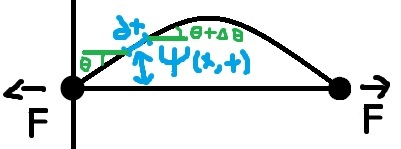
\includegraphics[width=0.6\textwidth]{figures/wave.jpg}
\caption{\label{fig:wave}This wave was uploaded via the project menu.}
\end{figure} \FloatBarrier

\subsection{Doppler effect}
\begin{tcolorbox}[breakable, enhanced]
\begin{align}
   \lambda^\prime = \lambda - u_s T = \lambda - \frac{u_s}{f}
\n f^\prime = \frac{V}{\lambda^\prime} = \frac{V}{\lambda - \frac{u_s}{f}} = f \left(\frac{1}{1 - \frac{u_s}{v}}\right) \eqComment{medium determines $V$}
\n  f^\prime = \frac{V^\prime}{\lambda} = \frac{V + u_r}{\lambda} = f (1 + \frac{u_r}{V}) \eqComment{wave determines $\lambda$}
\n f^\prime = \frac{V + u_r}{V + u_s} f \eqComment{general formula ?}
\end{align}
\end{tcolorbox}

\subsection{Wave interference and constrained waves}
\begin{tcolorbox}[breakable, enhanced]
\begin{align}
   \Psi_1 = A \cos(\omega_1 t) \eqSep \Psi_2 = A \cos(\omega_2 t)
\n \Psi = \Psi_1 + \Psi_2 = A (\cos(\omega_1 t) + \cos(\omega_2 t))
\n \Psi = (A) 2 \cos\left(\frac{\omega_1-\omega_2}{2} t\right) \cos\left(\frac{\omega_1+\omega_2}{2} t\right)
\n \omega_B = 2 \frac{\omega_1-\omega_2}{2} = \omega_1-\omega_2 \eqComment{$\cos(-x) = \cos(x)$}
\n A = \cos\left(\frac{2 \pi L_1}{\lambda}\right) + \cos\left(\frac{2 \pi L_2}{\lambda}\right) \eqComment{interference at a point and time}
\n L_1 - L_2 = \frac{\lambda}{2} \implies A = \cos\left(-\omega t + \frac{2 \pi L_1}{\lambda}\right) + \cos\left(-\omega t + \frac{2 \pi (L_1 - \frac{\lambda}{2})}{\lambda}\right) = \cos\left(-\omega t + \frac{2 \pi L_1}{\lambda}\right) +
\m \cos\left(-\omega t + \frac{2 \pi L_1}{\lambda} + \pi\right) = \cos\left(-\omega t + \frac{2 \pi L_1}{\lambda}\right) - \cos\left(-\omega t + \frac{2 \pi L_1}{\lambda}\right) = 0
\n L_1 - L_2 = 0 \implies A = \cos\left(-\omega t + \frac{2 \pi L_1}{\lambda}\right) + \cos\left(-\omega t + \frac{2 \pi L_1}{\lambda}\right) = 2 \cos\left(-\omega t + \frac{2 \pi L_1}{\lambda}\right) = 2 A_1
\n L_1 - L_2 = n \lambda \implies \textbf{constructive interference}
\n L_1 - L_2 = \left(n+\frac{1}{2}\right) \lambda \implies \textbf{destructive interference}
\n \left.\frac{d \Psi}{dt}\right|_{0 \land L} = 0 \implies f = \frac{V}{\lambda} = \frac{V}{\left(\frac{L}{n}\right)} = n \frac{V}{L} \eqComment{frequencies are quantized}
\end{align}
\end{tcolorbox}

\section{Fluid Mechanics}
\subsection{Density, pressure}
\begin{tcolorbox}[breakable, enhanced]
\begin{align}
   \rho = \frac{m}{V} = \frac{m}{r^3} \eqComment{density}
\n SI(\rho) = \frac{kg}{m^3}
\n P = \frac{F}{A} = \frac{F}{r^2} \eqComment{pressure}
\n SI(P) = \frac{N}{m^2} = \frac{kg}{m s^2} = \textbf{Pascals}
\n P_A = 10^3 \textbf{ Pascals}
\n P - P_A = P_g \eqComment{gauge pressure}
\end{align}
\end{tcolorbox}

\subsection{Fluid equilibrium}
\begin{tcolorbox}[breakable, enhanced]
\begin{align}
   P_{w_2} A - P_{w_1} A = 0
\n P_{w_2} = P_{w_1} \eqComment{points with the same depths have the same pressure}
\n P_{h_2} A - P_{h_1} A - A (h_2 - h_1) g \rho = 0
\n P_{h_2} = P_{h_1} + \rho g (h_2 - h_1) \eqComment{points with the different depths have different pressures}
\n P = P_A + \rho g h_A
\end{align}
\end{tcolorbox}

\subsection{Hydraulic press}
\begin{tcolorbox}[breakable, enhanced]
\begin{align}
   P_2 = P_1 = \frac{F_2}{A_2} = \frac{F_1}{A_1}
\n F_2 = F_1 \frac{A_2}{A_1} \eqComment{varying areas scales the output force}
\n W_2 = F_2 \Delta x_2 = P_2 A_2 \Delta x_2 = P_2 A_1 \Delta x_1 = P_1 A_1 \Delta x_1 = W_1
\end{align}
\end{tcolorbox}

\subsection{Buoyancy}
\begin{tcolorbox}[breakable, enhanced]
\begin{align}
   F_B = P_2 A - P_1 A = h A \rho g \eqComment{displaced weight}
\n \frac{V_s}{V} \rho_w g V - \rho g V = 0 \eqComment{equilibrium on water}
\n \frac{V_s}{V} = f_s = \frac{\rho}{\rho_w} \eqComment{fraction submerged in water}
\end{align}
\end{tcolorbox}

\subsection{Bernoulli's principle}
\begin{tcolorbox}[breakable, enhanced]
\begin{align}
   V_{\to 1} = V_{2 \to} \implies A_1 v_1 \Delta t = A_2 v_2 \Delta t \eqComment{incompressible fluids conserve internal system volume}
\n A_1 v_1 = A_2 v_2
\n E_2 = A_2 \Delta x_2 \rho \frac{{v_2}^2}{2} + A_2 \Delta x_2 \rho g h_2 = A_2 \Delta x_2 \rho \left(\frac{{v_2}^2}{2} + g h_2\right) \eqSep E_1 = A_1 \Delta x_1 \rho \left(\frac{{v_1}^2}{2} + g h_1\right)
\n W_2 = P_2 A_2 \Delta x_2 \eqSep W_1 = P_1 A_1 \Delta x_1
\n A_2 \Delta x_2 \rho \left(\frac{{v_2}^2}{2} + g h_2\right) - A_1 \Delta x_1 \rho \left(\frac{{v_1}^2}{2} + g h_1\right) = P_2 A_2 \Delta x_2 - P_1 A_1 \Delta x_1 \eqComment{Work-Energy theorem}
\n \frac{1}{dt} \left(A_2 \Delta x_2 \rho \left(\frac{{v_2}^2}{2} + g h_2\right) - A_1 \Delta x_1 \rho \left(\frac{{v_1}^2}{2} + g h_1\right)\right) = \frac{1}{dt} \left(P_2 A_2 \Delta x_2 - P_1 A_1 \Delta x_1\right)
\n A_2 v_2 \rho \left(\frac{{v_2}^2}{2} + g h_2\right) - A_1 v_1 \rho \left(\frac{{v_1}^2}{2} + g h_1\right) = P_2 A_2 v_2 - P_1 A_1 v_1 \eqSep A_1 v_1 = A_2 v_2
\n P_2 - P_1 = \rho \left(\frac{{v_2}^2}{2} + g h_2\right) - \rho \left(\frac{{v_1}^2}{2} + g h_1\right)
\n P_1 + \frac{\rho}{2} {v_1}^2 + \rho g h_1 = P_2 + \frac{\rho}{2} {v_2}^2 + \rho g h_2
\\ \Delta v \neq 0 \implies \Delta P \neq 0 \implies \Delta F \neq 0 \eqComment{varying flow rates produces a net force}
\end{align}
\end{tcolorbox}

\section{Thermodynamics}
\subsection{Temperature and ideal gas law}
\begin{tcolorbox}[breakable, enhanced]
\begin{align}
   T \eqComment{temperature}
\n SI(T) = K = \textbf{Kelvin}
\n \experimental 273.16 K = \textbf{water triple point} \eqSep 0 K = \textbf{absolute lowest temperature}
\n \experimental k = (1.38) 10^{-23} \frac{J}{K} \eqComment{Boltzmann constant}
\n N = \textbf{number of particles}
\n \experimental N_0 = (6.02) 10^{23} = \textbf{number of particles in $\frac{1 kg}{1000}$ of hydrogen} = \textbf{mole} \eqComment{Avogadro constant}
\n n = \frac{N}{N_0} = \textbf{number of moles}
\n R = N_0 k = 8.31 \frac{J}{K} \eqComment{gas constant}
\n \experimental P V = N k T = n R T \eqComment{ideal gas law independent of complex intermolecular forces}
\n F_{particle} = \frac{\Delta p}{\Delta t} = \frac{m v - (-m v)}{2 \frac{\sqrt[3]{V}}{v}} = \frac{2 m v}{\frac{2 L}{v}} = \frac{m v^2}{L}
\n F_\perp = \frac{N}{3} F_{particle} = \frac{N}{3} \left(\frac{m v^2}{L}\right)
\n P = \frac{F_\perp}{A} = \frac{N}{3} \left(\frac{m v^2}{L^3}\right) = \frac{N}{3} \left(\frac{m v^2}{V}\right)
\n P V = \frac{N}{3} m v^2 = N k T
\n \frac{m v^2}{2} = KE_g = \frac{3}{2} k T \eqComment{temperature as a measure of kinetic energy}
\n v \geq 0 \implies T \geq 0 \eqComment{existence of absolute zero temperature}
\end{align}
\end{tcolorbox}

\begin{figure}[h]
\centering
\begin{minipage}[b]{0.45\textwidth}
  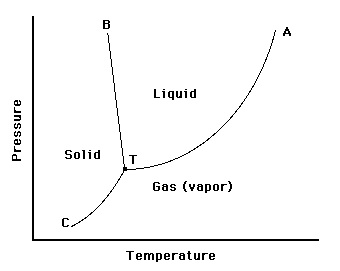
\includegraphics[width=\textwidth]{figures/triplepoint.jpg}
  \caption{\label{fig:triplepoint}This triplepoint was uploaded via the project menu.}
\end{minipage}
\hfill
\begin{minipage}[b]{0.45\textwidth}
  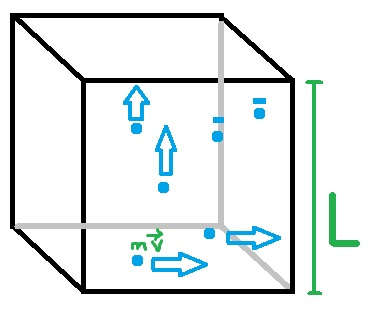
\includegraphics[width=\textwidth]{figures/microPV.jpg}
  \caption{\label{fig:microPV}This microPV was uploaded via the project menu.}
\end{minipage}
\end{figure} \FloatBarrier

\subsection{Heat and internal gas energy}
\begin{tcolorbox}[breakable, enhanced]
\begin{align}
   U = KE_g N = \frac{3}{2} N k T = \frac{3}{2} n R T = \frac{3}{2} P V \eqComment{internal energy}
\n \Delta U = \Delta Q - \Delta W = \Delta Q - F \Delta x = \Delta Q - P A \Delta x = \Delta Q - P \Delta V \eqComment{change in heat input and work output}
\end{align}
\end{tcolorbox}

\subsection{Specific heat}
\begin{tcolorbox}[breakable, enhanced]
\begin{align}
   n C = \frac{\Delta Q}{\Delta T} = \frac{\Delta U + P \Delta V}{\Delta T} \eqComment{controls the output $\Delta T$ per input $\Delta Q$}	
\n C_V = \left.\frac{dQ}{n dT}\right|_V = \frac{dU+0}{n dt} = \frac{3}{2} R
\n C_P = \left.\frac{dQ}{n dT}\right|_P = \left.\frac{dU + P dV}{n dT}\right|_P = C_V + \left.\frac{d(PV)}{n dT}\right|_P = C_V + \left.\frac{d(n R T)}{n dT}\right|_P = C_V + R = \frac{5}{2} R
\n \gamma = \frac{C_P}{C_V} = \frac{C_V + R}{C_V} = 1 + \frac{R}{C_V}
\n W_{cycle} = \oint P dV \neq 0 \eqComment{work of a state is undefined}
\n Q_{cycle} = \oint P dV \neq 0 \eqComment{heat of a state is undefined}
\n U_{cycle} = \oint P dV = 0 \eqComment{state variable}
\end{align}
\end{tcolorbox}

\subsection{Isothermal process}
\begin{tcolorbox}[breakable, enhanced]
\begin{align}
   \Delta T = 0 \implies \Delta  U = 0 \implies \Delta Q = \Delta W
\n W = \int_a^b P dV = n R T \int_a^b \frac{dV}{V} = n R T \ln\left(\frac{V_b}{V_a}\right)
\end{align}
\end{tcolorbox}

\subsection{Adiabatic process}
\begin{tcolorbox}[breakable, enhanced]
\begin{align}
   \Delta Q = 0 \implies 0 = \Delta U + P \Delta V = C_V n \Delta T + \frac{n R T}{V} \Delta V \eqComment{adiabatic process}
\n \frac{C_V}{R} \frac{\Delta T}{T} + \frac{\Delta V}{V} = 0
\n \frac{C_V}{R} \int_a^b \frac{dT}{T} + \int_a^b\frac{dV}{V} = 0 = \frac{C_V}{R} \ln\left(\frac{T_b}{T_a}\right) + \ln\left(\frac{V_b}{V_a}\right) = \ln\left(\left(\frac{T_b}{T_a}\right)^\frac{C_V}{R} \frac{V_b}{V_a}\right)
\n \left(\frac{T_b}{T_a}\right)^\frac{C_V}{R} \frac{V_b}{V_a} = 1
\n {T_b}^\frac{C_V}{R} V_b = {T_a}^\frac{C_V}{R} V_a
\n T_b {V_b}^\frac{R}{C_V} = T_a {V_a}^\frac{R}{C_V}
\n \frac{P_b V_b}{n R} {V_b}^\frac{R}{C_V} = \frac{P_a V_a}{n R} {V_a}^\frac{R}{C_V}
\n P_b {V_b}^\frac{1 + R}{C_V} = P_a {V_a}^\frac{1 + R}{C_V}
\n P_b {V_b}^\gamma = P_a {V_a}^\gamma = c
\n W = \int_a^b P dV = c \int_a^b\frac{dV}{V^\gamma} = c \int_a^b V^{-\gamma} dV = c \frac{{V_b}^{1 - \gamma} - {V_a}^{1 - \gamma}}{1 - \gamma} = \frac{P_b V_b^\gamma {V_b}^{1 - \gamma} - P_a V_a^\gamma {V_a}^{1 - \gamma}}{1 - \gamma} = 
\n \frac{P_b V_b - P_a V_a}{1 - \gamma} = \frac{P_a V_a - P_b V_b}{\gamma - 1} = \frac{\Delta(P V)}{1 - \gamma}
\end{align}
\end{tcolorbox}

\subsection{Heat engine}
\begin{tcolorbox}[breakable, enhanced]
\begin{align}
   W = Q_a - Q_b \eqComment{some heat is rejected}
\n \eta = \frac{W}{Q_a} = \frac{Q_a - Q_b}{Q_a} = 1 - \frac{Q_b}{Q_a} \eqComment{engine efficiency}
\n Q_h = n R T_h \ln\left(\frac{V_B}{V_A}\right)
\n Q_c = - n R T_c \ln\left(\frac{V_D}{V_C}\right) = n R T_c \ln\left(\frac{V_C}{V_D}\right)
\n \eta = 1 - \frac{T_c}{T_h} \frac{\ln(V_C / V_D)}{\ln(V_B / V_A)}
\n V_B {T_h}^\frac{C_V}{R} = V_C {T_c}^\frac{C_V}{R}
\n V_A {T_h}^\frac{C_V}{R} = V_D {T_c}^\frac{C_V}{R}
\n \frac{V_B}{V_A} = \frac{V_C}{V_D} \implies \frac{\ln(V_C / V_D)}{\ln(V_B / V_A)} = 1
\n \eta = 1 - \frac{Q_c}{Q_h} = 1 - \frac{T_c}{T_h} \eqComment{heat to work efficiency limit to reversible Carnot engine}
\end{align}
\end{tcolorbox}

\begin{figure}[h]
\centering
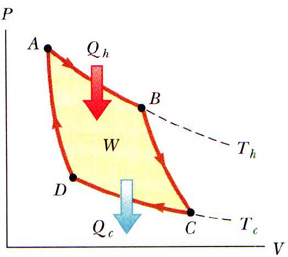
\includegraphics[width=0.6\textwidth]{figures/carnot.jpg}
\caption{\label{fig:carnot}This carnot was uploaded via the project menu.}
\end{figure} \FloatBarrier

\subsection{Theoretical heat engine efficiency limit}
\begin{tcolorbox}[breakable, enhanced]
\begin{align}
   \experimental Q_{hot}^{out} > Q_{hot}^{in} \eqComment{heat is not allowed to flow into a hotter system}
\n Q_{hot}^{out} = Q < \frac{\eta_M}{\eta_L} = Q_{hot}^{in} \eqComment{contradictory}
\n \sim \exists_E \eta_E > \eta_L
\end{align}
\end{tcolorbox}

\begin{figure}[h]
\centering
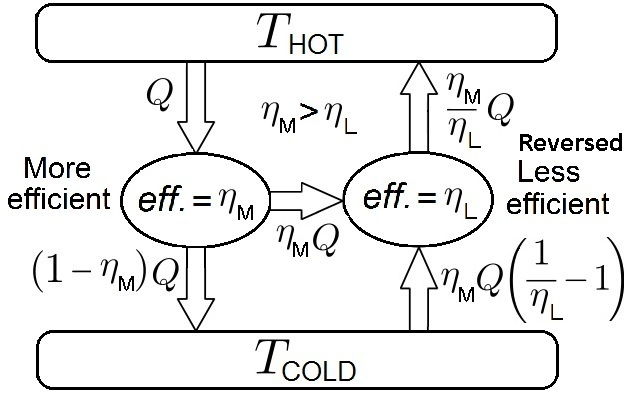
\includegraphics[width=0.6\textwidth]{figures/carnotengine.jpg}
\caption{\label{fig:carnotengine}This carnotengine was uploaded via the project menu.}
\end{figure} \FloatBarrier

\subsection{Entropy change}
\begin{tcolorbox}[breakable, enhanced]
\begin{align}
   \textbf{carnot cycle}
\n \sum_i \Delta Q_i = Q_h + 0 - Q_c - 0
\n \sum_i T_i = T_h + T_h - T_c - T_c
\n \sum_i \frac{\Delta Q_i}{T_i} = \frac{Q_h}{T_h} - \frac{Q_c}{T_c} = 0 = \sum_i \Delta S_i \eqComment{manufactured state variable entropy $S$}
\n \experimental \Delta S \geq 0 \eqComment{second law of thermodynamics}
\n \textbf{hot to cold heat transfer} \implies \Delta S = \frac{-Q}{T_h} + \frac{Q}{T_c} > 0 \implies \textbf{allowed}
\n \textbf{cold to hot heat transfer} \implies \Delta S = \frac{Q}{T_h} + \frac{-Q}{T_c} < 0 \implies \textbf{not allowed}
\n \textbf{hot and cold mixing} \implies \Delta S = n C (\int_{T_h}^{\frac{T_h + T_c}{2}}\frac{dT}{T} + \int_{T_c}^{\frac{T_h + T_c}{2}}\frac{dT}{T}) = n \ln\left(\frac{\left(\frac{T_h + T_c}{2}\right)^2}{T_h T_c}\right)
\n \left(\frac{T_h + T_c}{2}\right)^2 > T_h T_c \implies {T_h}^2 + 2 T_h T_c + {T_c}^2 > 4 T_h T_c \implies
\m {T_h}^2 - 2 T_h T_c + {T_c}^2 = (T_h - T_c)^2 > 0 \implies \Delta S > 0 \implies \textbf{allowed}
\n \textbf{hot and cold separating} \implies \Delta S = n C (\int_{\frac{T_h + T_c}{2}}^{T_h}\frac{dT}{T} + \int_{\frac{T_h + T_c}{2}}^{T_c}\frac{dT}{T}) < 0 \implies \textbf{not allowed}
\end{align}
\end{tcolorbox}

\subsection{Entropy}
\begin{tcolorbox}[breakable, enhanced]
\begin{align}
   \Delta T = 0 \implies Isothermal(S_1, S_2)
\n S_2 - S_1 = \Delta S = n R \ln\left(\frac{V_2}{V_1}\right)
\n V_2 = 2 V_1 \implies \Delta S = n R \ln\left(\frac{2 V_1}{V_1}\right) = n R \ln(2) = N k \ln(2) = k \ln(2^N)
\n \experimental S = k \ln(\Omega) \eqSep \Omega = \textbf{number of microstates satisfying the macrostate ?}
\n S_1 = k \ln(1)
\n S_2 - k \ln(2^N)
\n \textbf{dispersing gas} \implies S_2 - S_1 = \Delta S = k \ln(2^N) > 0 \implies \textbf{allowed}
\end{align}
\end{tcolorbox}

\begin{figure}[h]
\centering
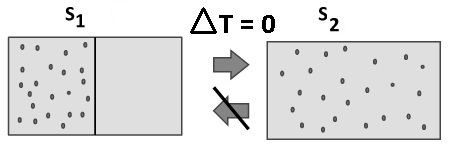
\includegraphics[width=0.6\textwidth]{figures/disorderstate.jpg}
\caption{\label{fig:disorderstate}This disorderstate was uploaded via the project menu.}
\end{figure} \FloatBarrier

\section{Electrodynamics}
\subsection{Electrical charge and field}
\begin{tcolorbox}[breakable, enhanced]
\begin{align}
   q \eqComment{electrical charge}
\n SI(q) = C = \textbf{Coulomb}
\n \experimental q_0 = (1.60) 10^{-19} C \eqComment{electron unit charge constant}
\n \experimental q_n = 0 C \eqComment{neutron electric charge}
\n \experimental q_e = -q_0 \eqComment{electron electric charge}
\n \experimental q_p = q_0 \eqComment{proton electric charge}
\n \experimental q = n q_0 \eqComment{electrical charge is quantized}
\n \experimental k_e = \frac{1}{4 \pi \epsilon_0} = (8.99) 10^9 \frac{N m^2}{C^2} \eqComment{electric force proportionality constant}
\n \experimental \vec{F_{2,1}} = \frac{q_2 q_1}{|\vec{r_2} - \vec{r_1}|^2} k_e \frac{\vec{r_2} - \vec{r_1}}{|\vec{r_2} - \vec{r_1}|} = \frac{q_2 q_1}{|\vec{r_2} - \vec{r_1}|^2} \frac{1}{4 \pi \epsilon_0} \frac{\vec{r_2} - \vec{r_1}}{|\vec{r_2} - \vec{r_1}|}  \eqComment{Coulomb's law}
\n \experimental \vec{F_i} = \sum_{j \neq i} \vec{F_{i,j}} \eqComment{classical charge superposition}
\n F_2 = \frac{q_1}{|\vec{r_2} - \vec{r_1}|^2} k_e \frac{\vec{r_2} - \vec{r_1}}{|\vec{r_2} - \vec{r_1}|} (q_2) = \vec{E}(\vec{r_2}) q_2 \eqComment{electric fields from external charges influences $q_2$}
\n \experimental \frac{\Delta q}{\Delta t} = 0 \eqComment{electrical charge conservation}
\end{align}
\end{tcolorbox}

\subsection{Dipole}
\begin{tcolorbox}[breakable, enhanced]
\begin{align}
   x(q_p) = a \land x(q_e) = -a \land y(q_p) = y(q_e) = 0 \implies E(x, 0) = 
\m \hat{x} q k_e \left(\frac{+1}{(x - a)^2} + \frac{-1}{(x + a)^2}\right) = \hat{x} q k_e \left(\frac{4 x a}{(x^2 - a^2)^2}\right) \eqComment{dipole system}
\n p = 2 q a \eqComment{dipole moment}
\n x >> a \implies E(x, 0) = \hat{x} q k_e \left(\frac{4 x a}{(x^2)^2}\right) = \hat{x} \frac{2 q a}{2 \pi \epsilon_0} \frac{1}{x^3} = \hat{x} \frac{p}{2 \pi \epsilon_0 x^3}
\n \vec{\tau} = \vec{F} \times \vec{d} = (E q) a (\sin(\theta) - \sin(\pi + \theta)) = E q a 2 \sin(\theta) = p E \sin(\theta) = \vec{p} \times \vec{E} \eqComment{dipole in uniform field}
\n U_\tau = -\int p E \sin(\theta) = -p E \cos(\theta) = p \cdot E
\end{align}
\end{tcolorbox}

\begin{figure}[h]
\centering
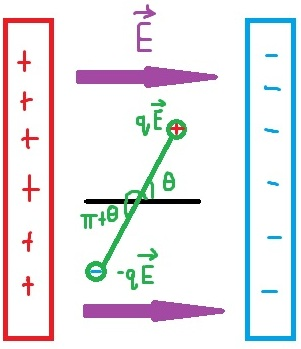
\includegraphics[width=0.35\textwidth]{figures/dipoleuniform.jpg}
\caption{\label{fig:dipoleuniform}This dipoleuniform was uploaded via the project menu.}
\end{figure} \FloatBarrier

\subsection{Infinite linear uniform charge}
\begin{tcolorbox}[breakable, enhanced]
\begin{align}
   \lambda \frac{C}{m} \eqComment{linear charge density}
\n dE = dE_y = \frac{\lambda dx k_e}{(\sqrt{x^2 + a^2})^2} \cos(\theta) = \frac{\lambda dx k_e}{x^2 + a^2} \frac{r_x(\theta)}{|r|} = \frac{\lambda dx k_e}{x^2 + a^2} \frac{a}{\sqrt{x^2 + a^2}}
\n E_y = \int_{-\infty}^\infty dE_y = \int_{-\infty}^\infty \frac{\lambda dx k_e}{x^2 + a^2} \frac{a}{\sqrt{x^2 + a^2}} = \lambda a k_e \int_{-\infty}^\infty \frac{dx}{(x^2 + a^2)^{3/2}}
\n x = a \tan(\theta) \implies \frac{dx}{d\theta} = a \sec^2{\theta} \implies dx = a \sec^2{\theta} d\theta
\n \int_{-\infty}^\infty \frac{dx}{(x^2 + a^2)^{3/2}} = \int_{-\frac{\pi}{2}}^{\frac{\pi}{2}} \frac{a \sec^2(\theta) d\theta}{((a \tan(\theta))^2 + a^2)^{3/2}} = \int_{-\frac{\pi}{2}}^{\frac{\pi}{2}} \frac{a \sec^2(\theta) d\theta}{(a^2 \tan^2(\theta) + a^2)^{3/2}} =
\m \int_{-\frac{\pi}{2}}^{\frac{\pi}{2}} \frac{a \sec^2(\theta) d\theta}{(a^2 (\tan^2(\theta) + 1))^{3/2}} = \int_{-\frac{\pi}{2}}^{\frac{\pi}{2}} \frac{a \sec^2(\theta) d\theta}{(a^2 \sec^2(\theta))^{3/2}} = \int_{-\frac{\pi}{2}}^{\frac{\pi}{2}} \frac{a \sec^2(\theta) d\theta}{a^3 \sec^3(\theta)} = \int_{-\frac{\pi}{2}}^{\frac{\pi}{2}} \frac{d\theta}{a^2 \sec^2(\theta)} =
\m \frac{1}{a^2} \int_{-\frac{\pi}{2}}^{\frac{\pi}{2}} d\theta \cos(\theta) = \frac{1}{a^2} \left.\sin(\theta)\right|_{-\frac{\pi}{2}}^{\frac{\pi}{2}} = \frac{1}{a^2} (1 - (-1)) = \frac{2}{a^2}
\n E = E_y = \lambda a k_e \frac{2}{a^2} = \frac{\lambda}{2 \pi \epsilon_0 a} \textbf{field strength falls linearly $1/a$}
\end{align}
\end{tcolorbox}

\begin{figure}[h]
\centering
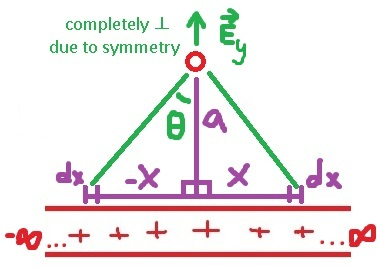
\includegraphics[width=0.6\textwidth]{figures/linearinfinitecharge.jpg}
\caption{\label{fig:linearinfinitecharge}This linearinfinitecharge was uploaded via the project menu.}
\end{figure} \FloatBarrier

\subsection{Infinite surface uniform charge}
\begin{tcolorbox}[breakable, enhanced]
\begin{align}
   \sigma \frac{C}{m^2} \eqComment{surface charge density}
\n dA = (2 \pi r) (dr)
\n dE = dE_z = \frac{\sigma dA k_e}{r^2 + a^2} \frac{a}{(r^2 + a^2)^{1/2}} = \frac{\sigma 2 \pi r dr k_e}{r^2 + a^2} \frac{a}{(r^2 + a^2)^{1/2}}
\n E_z = \int_0^\infty dE_z = \int_0^\infty \frac{(2 \pi \sigma a k_e) r dr}{(r^2 + a^2)^{3/2}} = \frac{\sigma a}{4 \epsilon_0} \int_0^\infty \frac{2 r dr}{(r^2 + a^2)^{3/2}}
\n u = r^2 \implies \frac{du}{dr} = 2 r \implies du = 2 r dr
\n \int_0^\infty \frac{du}{(u + a^2)^{3/2}} = \left.(u + a^2)^{-1/2} \left(\frac{-2}{1}\right)\right|_0^\infty = 0 - \frac{-2}{a^2} = \frac{2}{a^2}
\n E = E_z = \frac{\sigma a}{4 \epsilon_0} \left(\frac{2}{a^2}\right) = \frac{\sigma}{2 \epsilon_0}
\end{align}
\end{tcolorbox}

\subsection{Gauss's law}
\begin{tcolorbox}[breakable, enhanced]
\begin{align}
   S = \textbf{sphere} \implies A = 4 \pi r^2
\n d\vec{A} = dA \hat{\perp}(A)
\n \vec{E} = \frac{q}{4 \pi \epsilon_0} \frac{1}{r^2} \frac{\vec{r}}{r} = \frac{q}{4 \pi \epsilon_0} \frac{1}{r^2} \hat{r}
\n S \implies \hat{r} \parallel \hat{\perp}(A) \implies \vec{E} \cdot d\vec{A} = E dA \cos(\theta) = d\vec{A} = E dA \cos(0) = E dA \eqComment{alternatively ...}
\n \vec{E} \cdot d\vec{A} = \frac{q dA}{4 \pi \epsilon_0 r^2} \left(\hat{r} \cdot \hat{\perp}(A)\right) = \frac{q dA}{4 \pi \epsilon_0 r^2} \eqComment{amount flow across a small area}
\n \phi_{sphere} = \int \vec{E} \cdot d\vec{A} = \frac{q}{4 \pi \epsilon_0 r^2} \int dA = \frac{q}{4 \pi \epsilon_0 r^2} A = \frac{q}{\epsilon_0} \eqComment{electric flow or flux through spherical surface}
\n S = \textbf{closed surface}
\n V \eqComment{enclosed volume} \eqSep \partial V \eqComment{volume boundary or surface area}
\n \iint\limits_S \vec{E_1 + E_2} \cdot d\vec{A} = \iint\limits_S \vec{E_1} \cdot d\vec{A} + \vec{E_2} \cdot d\vec{A} = \frac{q_1 + q_2}{\epsilon_0} \eqComment{superposition}
\n q_V = \sum\limits_{i \in V} q_i
\n \phi = \varoiint\limits_{S = \partial V} \vec{E} \cdot d\vec{A} = \frac{q_V}{\epsilon_0}\eqComment{electric flux due to a discrete charge distribution}
\n \rho \eqComment{charge density} \eqSep SI(\rho) = \frac{C}{m^3}
\n \varoiint\limits_{S=\partial V} \vec{E} \cdot d\vec{A} = \iiint\limits_V \rho(x,y,z) dx dy dz \eqComment{electric flux due to a continuous charge distribution}
\end{align}
\end{tcolorbox}

\subsection{Solid charged sphere}
\begin{tcolorbox}[breakable, enhanced]
\begin{align}
   S = \textbf{sphere}
\n \phi = E 4 \pi r^2 = \frac{q_V}{\epsilon_0}
\n \vec{E}(\vec{r}) = \hat{r} \frac{q_V}{4 \pi \epsilon_0} \frac{1}{r^2} 
\n r_{in} \leq r
\n V(r) = \frac{4}{3} \pi r^3 \eqComment{volume of a sphere}
\n \vec{E}(\vec{r_{in}}) = \frac{\hat{r_{in}}}{4 \pi {r_{in}}^2 \epsilon_0} \frac{q_V}{V(r)} V(r_{in}) = \frac{\hat{r_{in}}}{4 \pi r{_{in}}^2 \epsilon_0} \frac{q_V {r_{in}}^3}{r^3} = \hat{r_{in}} \frac{q_V}{4 \pi \epsilon_0} \frac{r_{in}}{r^3} \eqComment{increases with $r_{in}$}
\end{align}
\end{tcolorbox}

\subsection{Hollow charged sphere}
\begin{tcolorbox}[breakable, enhanced]
\begin{align} % TODO figure cone in sphere
   A(r) = \frac{c}{r^2} \eqComment{area of a circular cone base}
\n \sigma \frac{A_1}{{r_1}^2} = \sigma c = \sigma \frac{A_2}{{r_2}^2} \eqComment{charges on from opposing sides cancel}
\end{align}
\end{tcolorbox}

%% CURRENT LECTURE: 2.4;0:44:50

%%%%% APPENDIX %%%%%
Note: RHS is based on the external normal of a closed surface lolol.

%%%%%%%%%%%%%%%%%%%%%%%%%%%%%%%%%%%
%%%%%%%%%%%%%%%%%%%%%%%%%%%%%%%%%%%
%%%%%%%%%%%%%%%%%%%%%%%%%%%%%%%%%%%
%%%%%%%%%%%%%%%%%%%%%%%%%%%%%%%%%%%
%%%%%%%%%%%%%%%%%%%%%%%%%%%%%%%%%%%
%%%%%%%%%%%%%%%%%%%%%%%%%%%%%%%%%%%
%%%%%%%%%%%%%%%%%%%%%%%%%%%%%%%%%%%
%%%%%%%%%%%%%%%%%%%%%%%%%%%%%%%%%%%
%%%%%%%%%%%%%%%%%%%%%%%%%%%%%%%%%%%
%%%%%%%%%%%%%%%%%%%%%%%%%%%%%%%%%%%
%%%%%%%%%%%%%%%%%%%%%%%%%%%%%%%%%%%
%%%%%%%%%%%%%%%%%%%%%%%%%%%%%%%%%%%
\bibliography{sample}
% Walter Greiner - Thermodynamics and statistical mechanics : http://home.basu.ac.ir/~psu/Books/stat%20thermo%20Greiner.pdf
% Shankar's Fundamentals of Physics 1 & 2
% rudin + lectures
\end{document}
